V této studii bylo zkoumáno 5 různých nodalizací termohydraulického modelu reaktoru VR-1 v programu RELAP5. V této kapitole jsou všechny modely srovnány mezi sebou, porovnány s daty z reaktoru Triga Mark II a okomentovány v souvislosti s bezpečnostními analýzami.

Z analýzy vyplynulo, že referenční model (NOD00) a renodalizovaný model NOD02 mají odlišné chování v porovnání s modely NOD01 a NOD04. Tyto modely neumožňují vzniku recirkulace ve volném objemu na AZ v horizontálním obtoku a dochází k nadhodnocení celkového průtoku (komentář k této problematice je uveden v kapitole \ref{chap:th_model_vr_1}). Toto nadhodnocení vede díky lepšímu odvodu tepla k celkově nižší výstupní teplotě chladiva. Pro kontext  jsou na obr. \ref{fig:cfd_triga_temperatures_velocities} uvedeny grafy využité k validaci termohydraulického CFD modelu reaktoru TRIGA Mark I \cite{TRIGA_CFD}. V \cite{TRIGA_CFD} je předpokládán přechodový jev (exkurze výkonu na konstantní hodnotu) za vzniku ustáleného přirozeného proudění, detailní průběh výkonu ale není doložen. Chování průměrných teplot a rychlostí v AZ reaktoru TRIGA lze vztáhnout k výsledkům uvedeným na obr. \ref{fig:G_stationary_100} a \ref{fig:T_out_stationary_100}.


\begin{figure}[H]
	\centering
	\begin{minipage}{.5\textwidth}
		\centering
		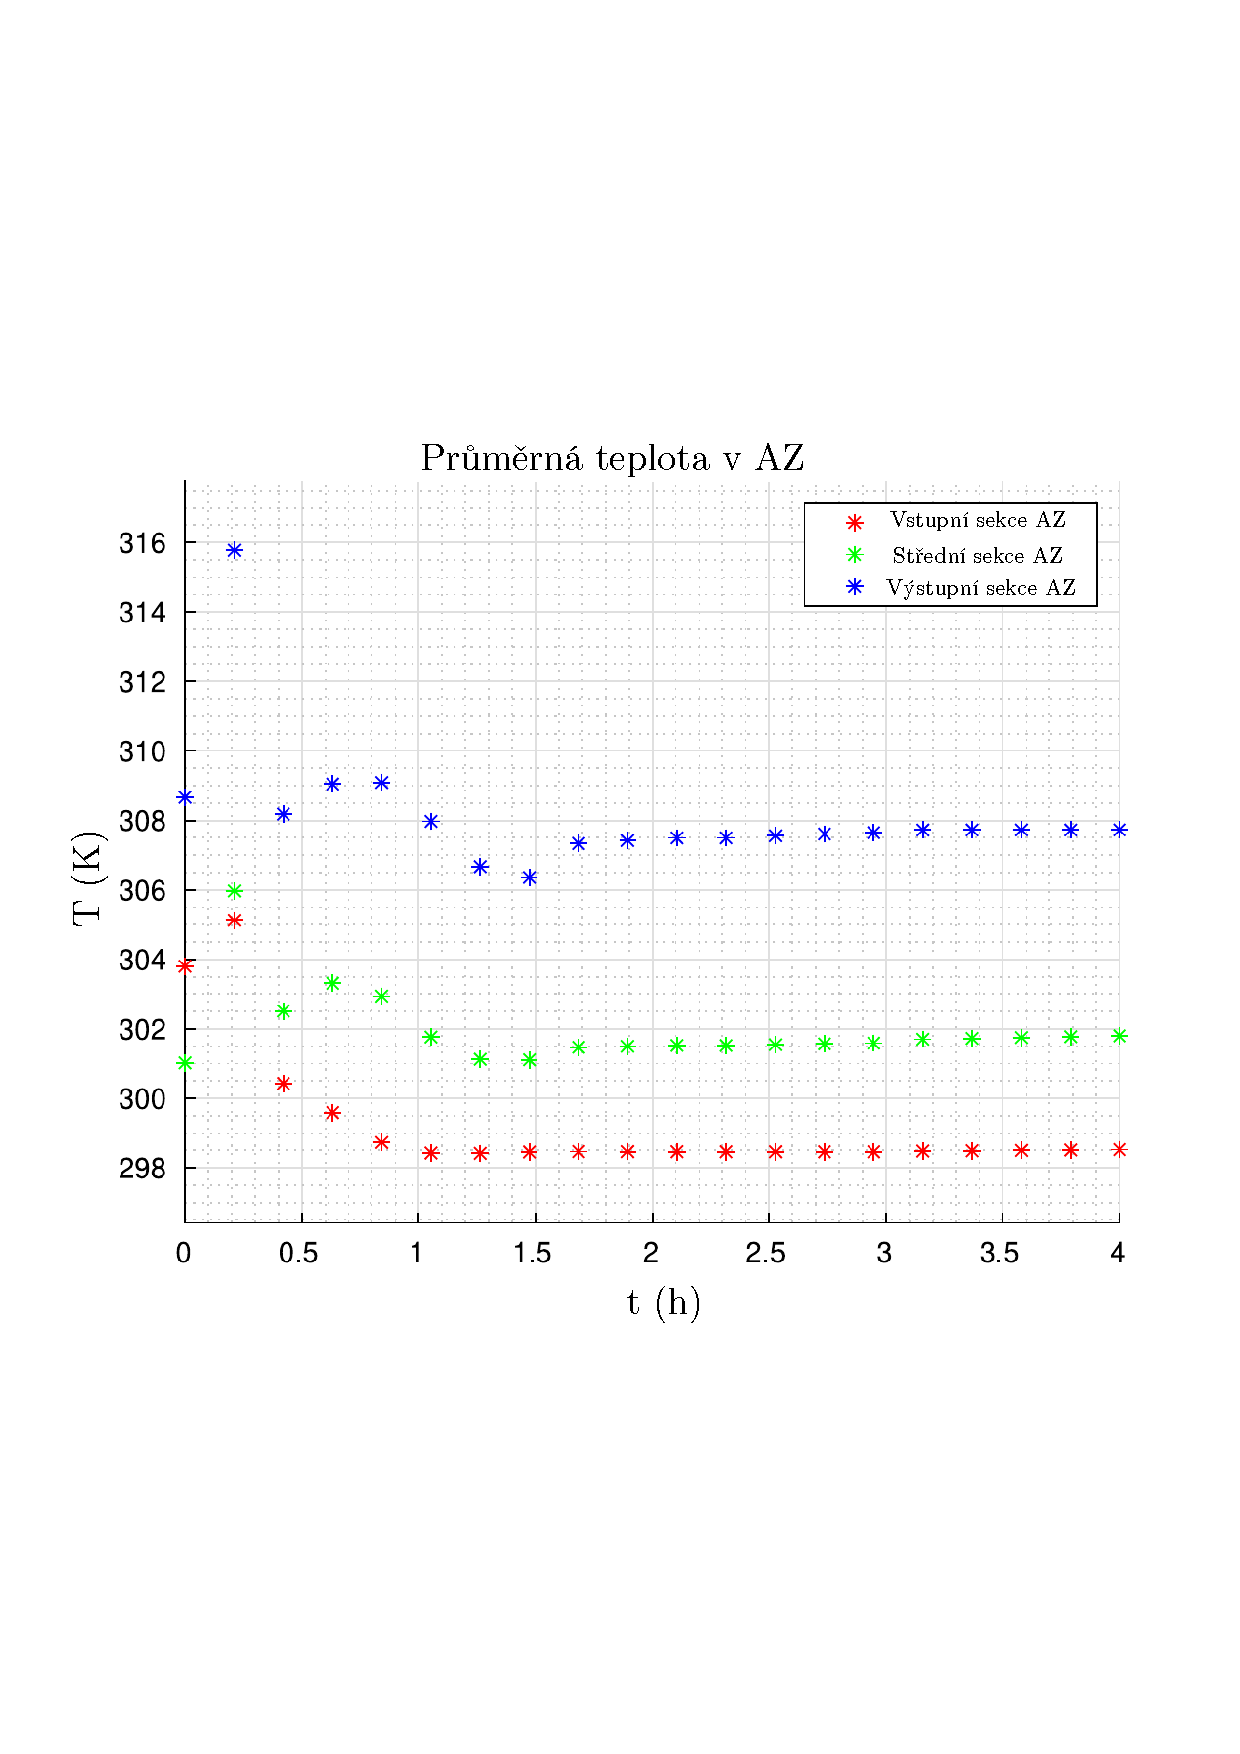
\includegraphics[width=\textwidth, trim={1cm 7cm 1cm 7cm}, clip]{./06_hodnoceni_TH_modelu/obrazky/cfd_triga_temperatures.pdf}
%		\caption{teploty}
%		\label{fig:cfd_triga_temperatures}
	\end{minipage}%
	\begin{minipage}{.5\textwidth}
		\centering
		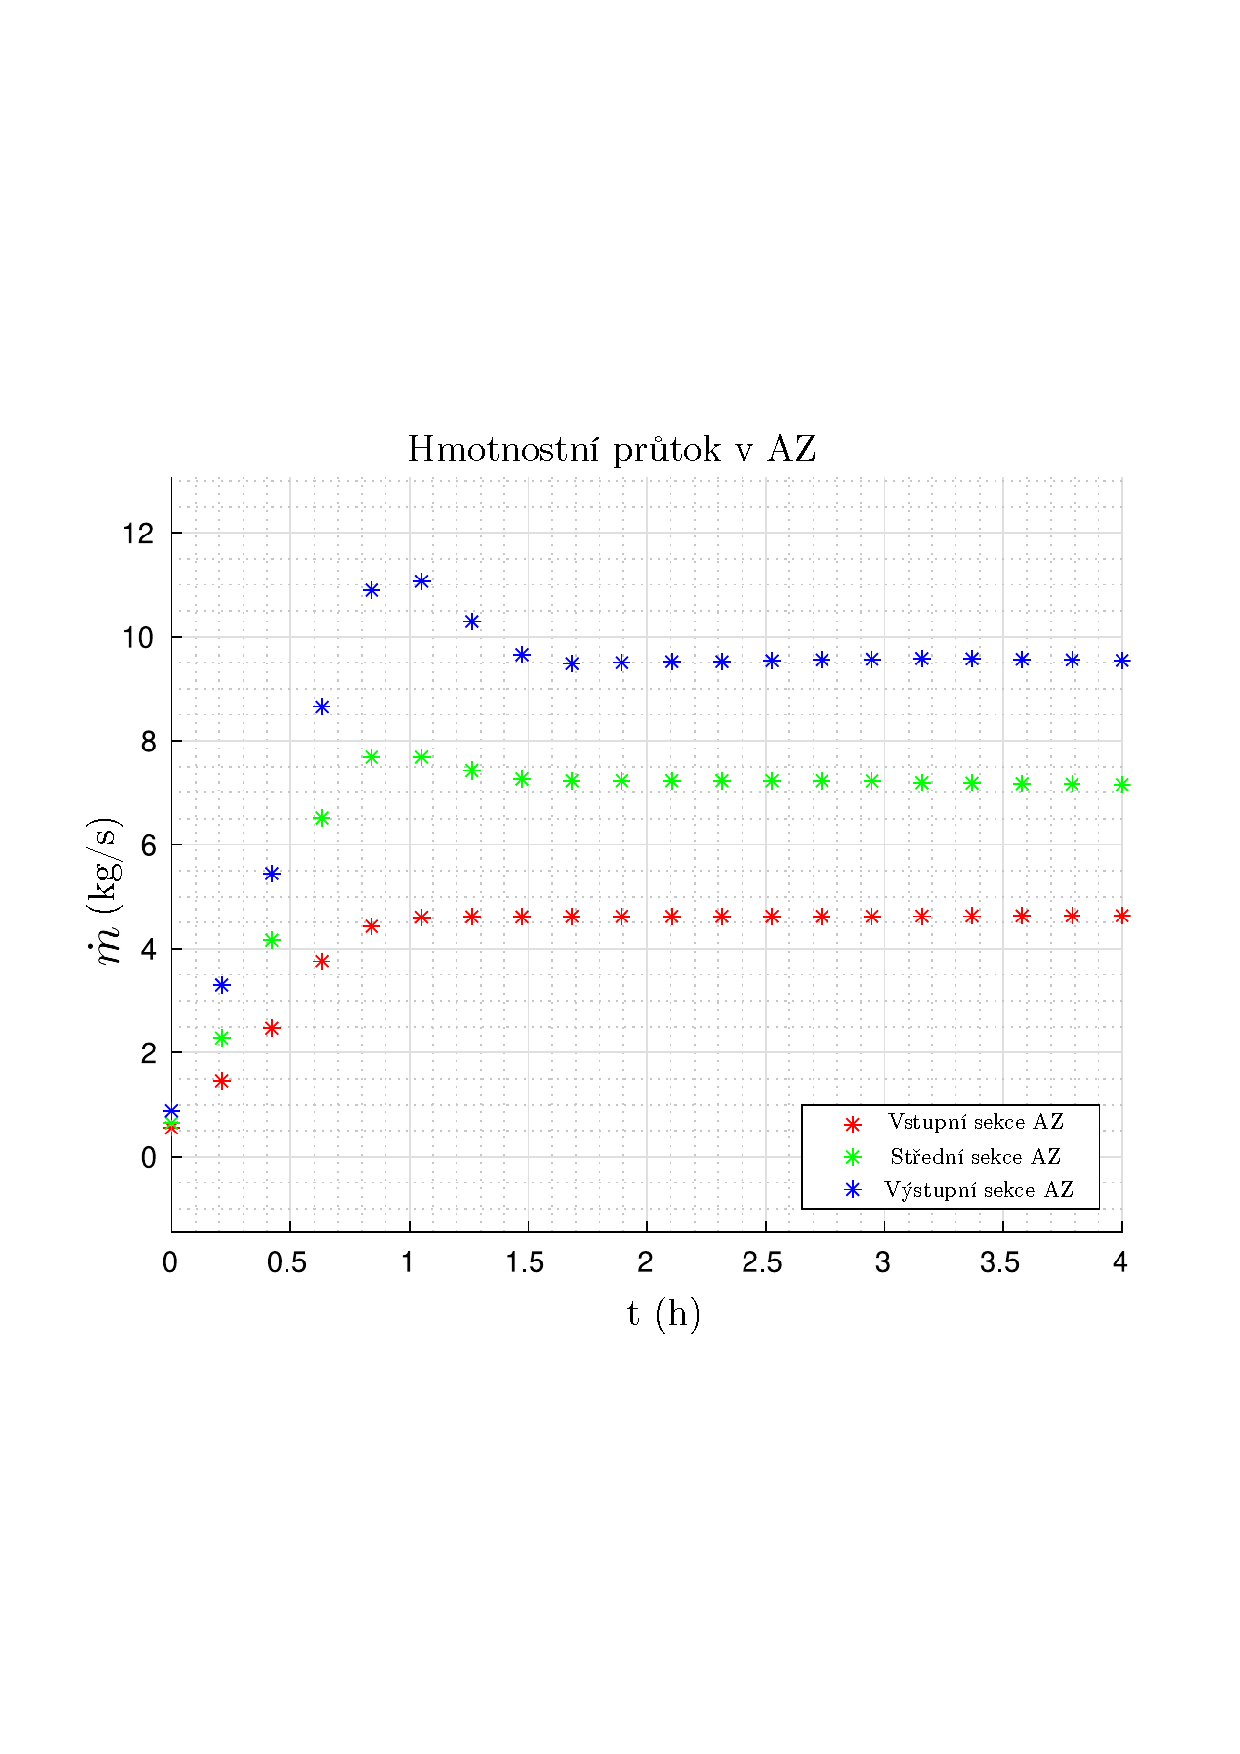
\includegraphics[width=\linewidth, trim={1cm 7cm 1cm 7cm}, clip]{./06_hodnoceni_TH_modelu/obrazky/cfd_triga_mass_flow_rate.pdf}
%		\caption{Průměrné rychlosti}
%		\label{fig:cfd_triga_mass_flow_rate}
	\end{minipage}
	\caption{Průměrné teploty a rychlosti v jednotlivých částech AZ reaktoru TRIGA Mark II (CFD výpočet) \cite{TRIGA_CFD}.}
	\label{fig:cfd_triga_temperatures_velocities}
\end{figure}
\begin{figure}[H]
	\centering
	\begin{minipage}{.5\textwidth}
		\centering
		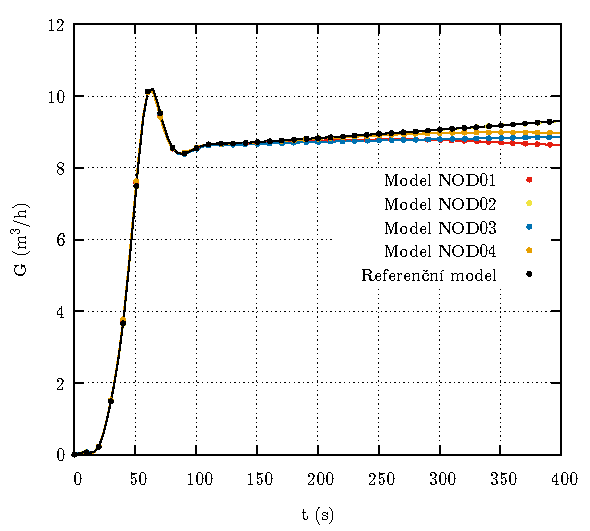
\includegraphics[width=\textwidth]{./06_hodnoceni_TH_modelu/grafy/G_stationary_100_trans.pdf}
%		\caption{Přechodový stav.}
%		\label{fig:G_stationary_100_trans}
	\end{minipage}%
	\begin{minipage}{.5\textwidth}
		\centering
		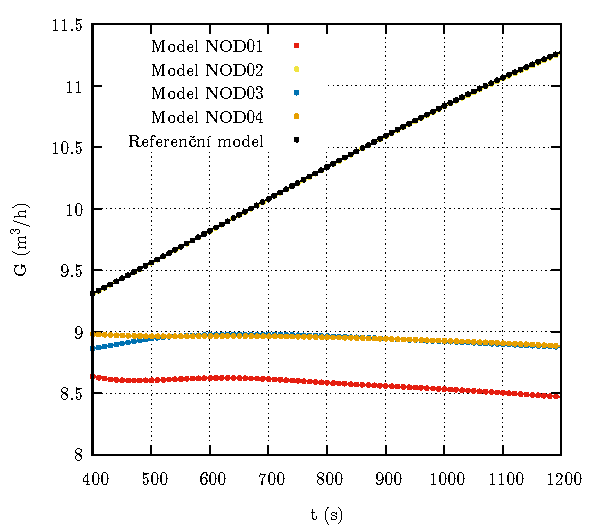
\includegraphics[width=\linewidth]{./06_hodnoceni_TH_modelu/grafy/G_stationary_100.pdf}
%		\caption{Kvazistacionární stav.}
		
	\end{minipage}
	\caption{Průtok skrz AZ reaktoru VR-1 pro jednotlivé modely (RELAP5).}
	\label{fig:G_stationary_100}
\end{figure}

Z porovnání obr. \ref{fig:G_stationary_100} lze soudit, že průtok v referenčním modelu a modelu NOD02 neodpovídá chování CFD výpočtu uvedenému na obr. \ref{fig:cfd_triga_temperatures_velocities}. Vzhledem k vyššímu průtoku a tedy lepšímu odvodu tepla se modely NOD00 a NOD02 jeví jako méně konzervativní. Proto by pro výpočet přechodových jevů v rámci bezpečnostních analýz bylo vhodnější využít modely NOD01 a NOD04, které mají nižší a konstantní průtok a tedy se zdají být konzervativnější a stabilnější. Z důvodu nestability popsané v sekci \ref{sec:nod_03} (špatné konstrukce vodní hladiny) není vhodné používat model NOD03 pro další analýzy.

Teplota na výstupu z AZ je nejvyšší v případě modelu NOD01, tedy model se pro analýzu přechodových jevů zdá být v rámci zkoumaných modelů nejvíce konzervativní.
\begin{figure}[H]
	\centering
	\begin{minipage}{.5\textwidth}
		\centering
		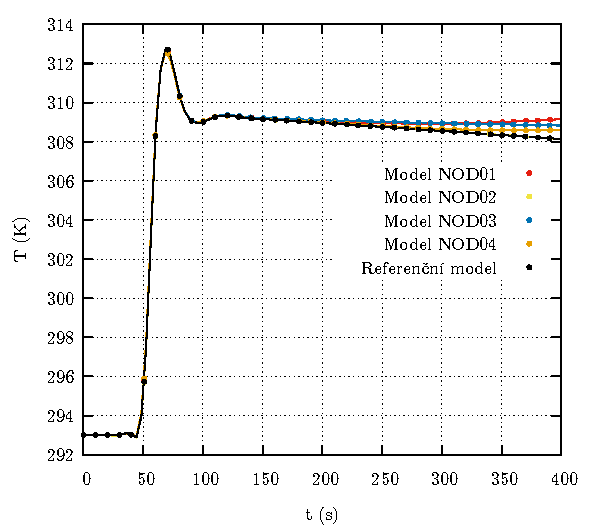
\includegraphics[width=\textwidth]{./06_hodnoceni_TH_modelu/grafy/T_out_stationary_100_trans.pdf}
		%		\caption{Přechodový stav.}
		%		\label{fig:T_out_stationary_100_trans}
	\end{minipage}%
	\begin{minipage}{.5\textwidth}
		\centering
		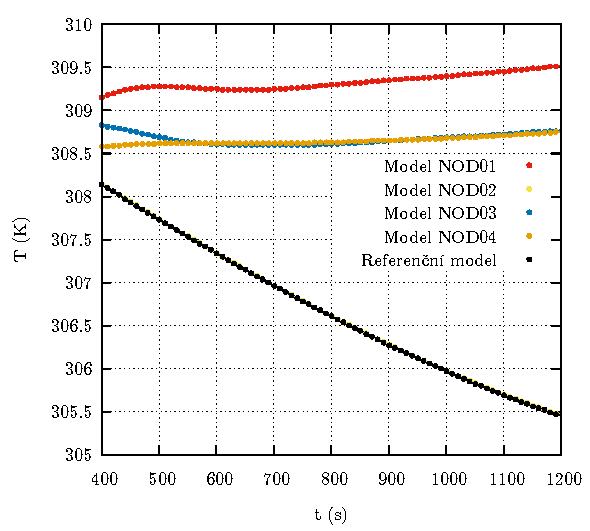
\includegraphics[width=\linewidth]{./06_hodnoceni_TH_modelu/grafy/T_out_stationary_100.pdf}
		%		\caption{Kvazistacionární stav.}
		
	\end{minipage}
	\caption{Teploty chladiva na výstupu z AZ reaktoru VR-1 pro jednotlivé modely (RELAP5).}
	\label{fig:T_out_stationary_100}
\end{figure}




\begin{figure}[H]
	\centering
	\begin{minipage}{.5\textwidth}
		\centering
		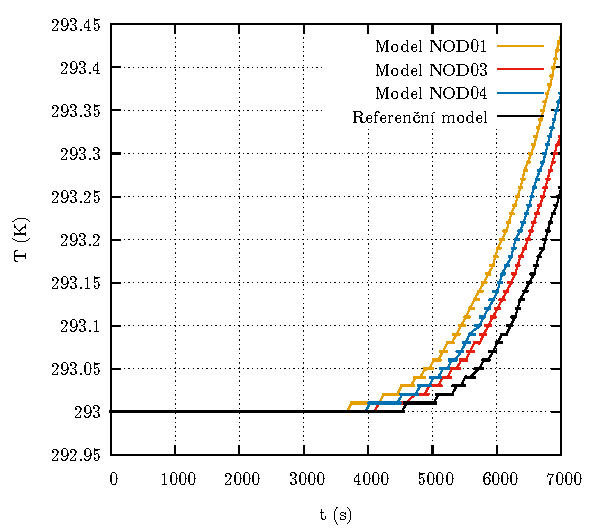
\includegraphics[width=\textwidth]{./06_hodnoceni_TH_modelu/grafy/T_in_stationary_102_long.pdf}
		\caption{Vstupní teplota chladiva pro jednotlivé modely (RELAP5)}
		\label{fig:T_in_stationary_102_long}
	\end{minipage}%
	\begin{minipage}{.5\textwidth}
		\centering
		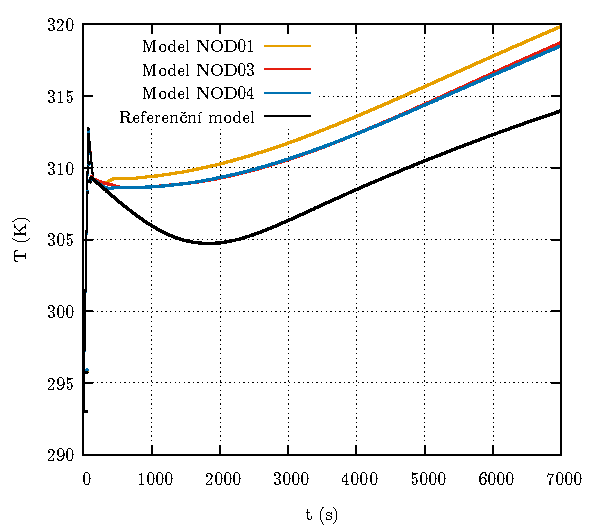
\includegraphics[width=\linewidth]{./06_hodnoceni_TH_modelu/grafy/T_out_stationary_100_long.pdf}
		\caption{Výstupní teplota chladiva pro jednotlivé modely (RELAP5).}
		\label{fig:T_out_stationary_100_long}
	\end{minipage}
	
\end{figure}

Dále platí, že doba, než dojde k úplné recirkulaci a tedy k nárůstu teploty na vstupu do AZ, je nejnižší u modelů NOD03 a NOD04. Tato skutečnost vyplývá z obr. \ref{fig:T_in_stationary_102_long}. Po dobu kolem 4000 s je vstupní teplota chladiva konstantní. Následně dochází ke schodovitému nárůstu, u kterého lze spekulovat o fyzikálním odůvodnění. Čas 4000 s ovšem odpovídá rychlosti proudění a konstrukci reaktoru, tedy jako původ tohoto nárůstu lze považovat vstup ohřáté kapaliny do AZ. Model NOD02 není uveden, neboť má identické chování jako referenční model.

\begin{figure}[H]
 	\centering
 	\begin{minipage}{.5\textwidth}
 		\centering
 		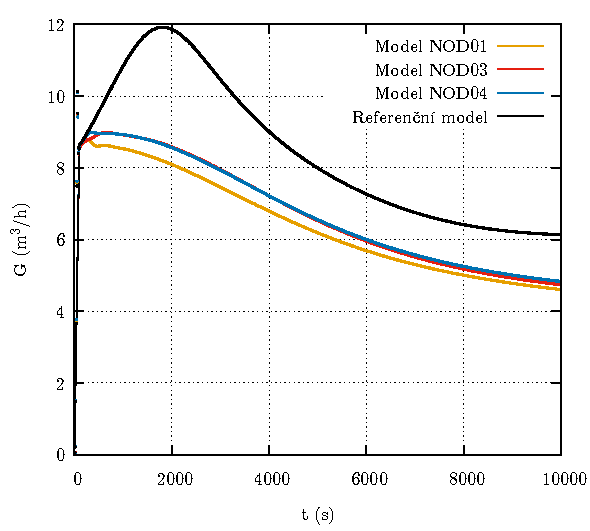
\includegraphics[width=\textwidth]{./06_hodnoceni_TH_modelu/grafy/G_stationary_100_long.pdf}
 		
 	\end{minipage}%
 	
 	\caption{Průtok skrz AZ reaktoru VR-1 pro jednotlivé modely (RELAP5).}
 	\label{fig:G_stationary_100_long}
\end{figure}

Ohřev celkového objemu v reaktorové nádobě vede u všech modelů k poklesu teplotního gradientu a tedy i ke klesajícímu průtoku viz obr. \ref{fig:G_stationary_100_long}. 



Pro úplnost jsou v tab. \ref{tab:teploty_hs} uvedeny průměrné a maximální teploty HS pro jednotlivé modely. Opět se jako nejkonzervativnější jeví model NOD01, kdy je průměrná a maximální teplota HS nejvyšší. V rámci výpočtů lze ovšem rozdíly mezi jednotlivými modely považovat za zanedbatelné.
\begin{table}[H]
	\centering
	\caption{Maximální a průměerné teploty HS pro jednotlivé modely.}
	\label{tab:teploty_hs}
	\begin{tabular}{ccc}
		\hline
		Model	&	$ T_{\text{av}} $ (K)	& $ T_{\text{max}} $ (K)	\\
		\hline
		\hline
		NOD00	&	308,7	&	 313,6	 \\
		NOD01	&	309,5	&	 314,9	 \\
		NOD02	&	308,7	&	 313,6	 \\
		NOD03	& 	309,2	&	 314,4	 \\
		NOD04	&	309,2	&	 314,3	 \\
		\hline
	\end{tabular}
\end{table} 





Celkově z uvedených výsledků vyplývá, že jako vhodné pro analýzu přechodových se jeví renodalizované termohydraulické modely NOD01 a NOD04. V obou případech je charakteristika přirozeného proudění stabilní a chováním odpovídá \cite{TRIGA_CFD}. Pro bezpečnostní analýzy se může zdát vhodnější model NOD01, který je v porovnání s ostatními modely nejkonzervativnější.




%\begin{figure}[H]
%	\centering
%	\begin{minipage}{.5\textwidth}
%		\centering
%		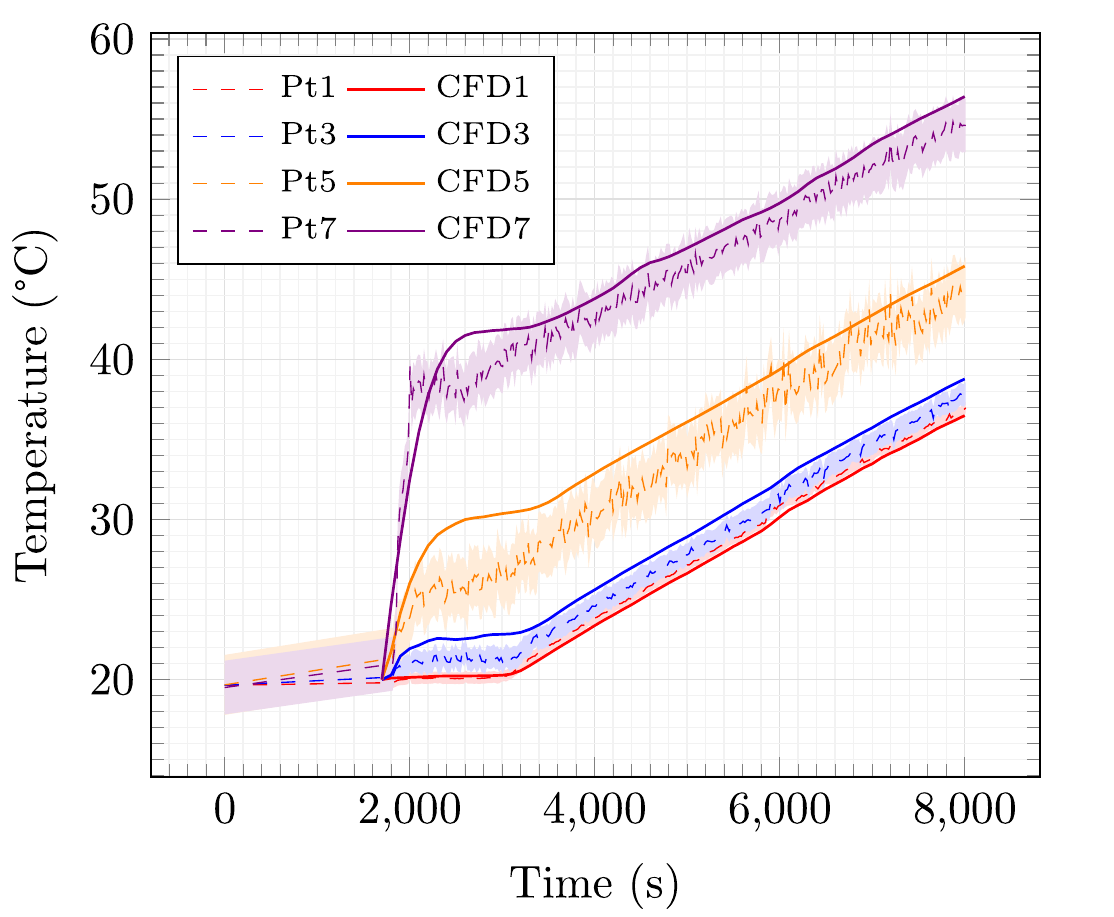
\includegraphics[width=\textwidth]{./06_hodnoceni_TH_modelu/obrazky/cfd_triga_temperatures_az_odd.png}
%		\caption{Lichá sada termočlánků.}
%		\label{fig:cfd_triga_temperatures_az_odd}
%	\end{minipage}%
%	\begin{minipage}{.5\textwidth}
%		\centering
%		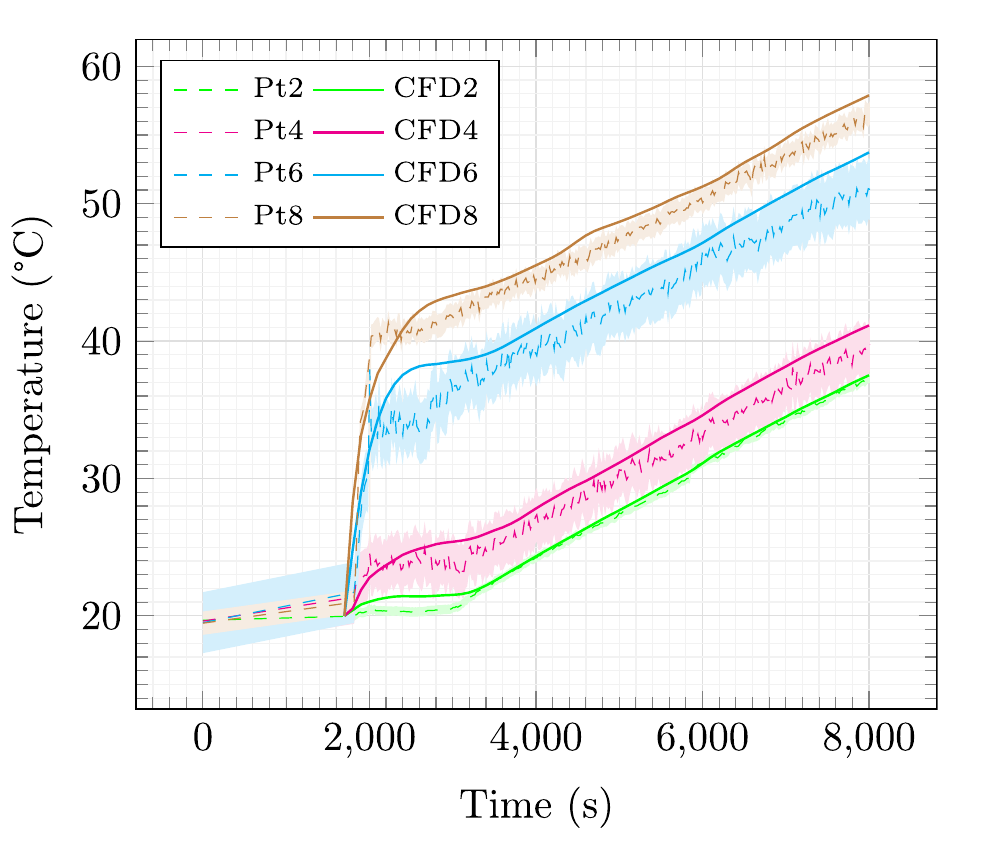
\includegraphics[width=\linewidth]{./06_hodnoceni_TH_modelu/obrazky/cfd_triga_temperatures_az_even.png}
%		\caption{Sudá sada termočlánků.}
%		\label{fig:cfd_triga_temperatures_az_even}
%	\end{minipage}
%	\caption{Teploty v jednotlivých částech AZ reaktoru TRIGA Mark II - (Experiment a CFD výpočet) \cite{TRIGA_CFD}.}
%\end{figure}



